% !TeX root = ../../thesis.tex
\chapter{Phase field method}

\section{Basic information}
Phase field method is a diffuse-interface approach to solving moving-boundary problems, in materials science usually perceived as a meso-scale method. It has numerous applications such as e.g. (multi-component) solidification, grain growth, Ostwald ripening, solid-solid phase transitions (martensitic, precipitation, spinodal...), two-phase flow, nucleation and much more. 

A phase (or phases) in an inhomogeneous system is described by a continuous function (called phase field), having different constant values in the bulk of the phases (typically 1 and 0 or 1 and -1). At the interface between phases, the phase field varies smoothly between the values and the interface region is thus characterized by a certain width, as sketched in Figure~\ref{fig_PFintro_diffuse_interface}. This interface width is an important input parameter in phase field models. In quantitative phase field models, the model behavior is in principle not affected by the particular value of interface width chosen, which allows to make quantitative simulations at mesoscale (the real interface width would require unfeasibly fine simulation grids).

\begin{figure}
	\centering
	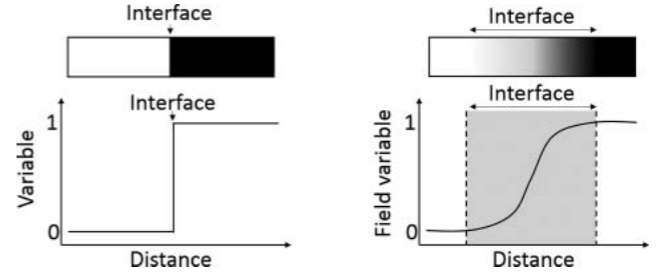
\includegraphics[width = 0.6\textwidth]{chapters/03PFintro/image/diffuse_interface_Bellemans2017}
	\caption{Illustration of the diffuse interface in phase field method (on the right) and the comparison to an actual, sharp interface (on the left).~\cite{Bellemans2017}}
	\label{fig_PFintro_diffuse_interface}
\end{figure}

Usually, the phases evolve in systems with bulk physical fields like concentration, temperature or other ones. These also contribute to the energy of the system. The total energy is defined as a functional on a space of functions inhabitated by the phase fields and the physical fields describing the system. The coupled governing equations describing evolution of each of the phase fields can be derived from the free energy functional using principles of variational calculus. Qualitatively speaking, the equations are constructed in such a way, that the system evolves along the 'direction of steepest descent' in energy so that the free energy is minimized, i.e. the equilibrium reached. 

The governing equations for the phase fields are typically either conservative (Cahn-Hilliard type of equation, conserving volume) or non-conservative (Allen-Cahn type of equation). The latter is more relevant for this work. The Alen-Cahn equation describing evolution of a non-conserved field $\eta(\mathbf{r})$ in a domain $\Omega\in\mathbb{R}^3$ with boundary $\partial\Omega$ can be written as
\begin{align}
	\frac{\partial \eta}{\partial t} = -L\frac{\delta F}{\delta \eta} \quad &\mathrm{in \,\Omega}\\
	\nabla\eta\cdot\bm{n} = 0 \quad &\mathrm{at \, \partial\Omega}\,,
\end{align}
where $L$ is a positive constant and the function $\frac{\delta F}{\delta \eta}$ stands for functional derivative of the free energy functional $F$. The latter expresses how much the energy changes when the function $\eta(\mathbf{r})$ is infinitesimally varied. It was shown that the Allen-Cahn equation with the following free energy functional is a diffuse-interface approximation of curvature-driven system
\begin{equation}
	F = \int_V m \eta^2(1-\eta)^2 - \kappa|\nabla\eta|^2 \mathrm{d}V
\end{equation}

Phase field method is in principle highly versatile, because it is readily extensible by inclusion of new physical fields in the free energy density and by adding the respective governing equation to the present system.

{\color{red}{GO ON HERE - formulas for IW, IE, governing equation}}

there is an expression for the free energy density of the system as function of the fields of interest, their evolution can in principle be simulated with this approach.

Due to the thermodynamic nature of the method, the interface energy is naturally included as an input parameter. Multigrain or multiphase systems with interfaces of various properties can be simulated with multi phase field models. Some of these allow to include also inclination dependence of interface energy. In fact, it was phase field simulation which revealed the paramount importance of interface energy anisotropy in pattern formation during dendritic solidification.
\begin{itemize}
	\item thermodynamic reasonong, free energy functional, diffuse interface
	\item Allen-Cahn equation and curvature driving force
	\item some historical context
	\item applications, coupling of physics
\end{itemize}

\section{Multi-phase field models with anisotropic interface energy}
Bring here stuff from the Paper1.
\begin{itemize}
	\item natural vs classical formulation
\end{itemize}
Grain coarsening is assumed to be curvature-driven, hence it is an appealing application for only-interface-driven multi-phase field models. Real interfaces (including the grain boundaries) exhibit anisotropic (inclination-dependent) interface energies ~\cite{Olmsted2009,Bulatov2014}, hence a significant effort was made to introduce this feature in some multi-phase field models too~\cite{Garcke1999,Toth2015,Salama2020,Kazaryan2000,Wendler2011}.

The models have different formulations, but the differences in their behavior are not obvious, especially because there is no unified validation procedure for quantitative comparison. Systematic and reproducible parametric studies in well-defined problems are needed for quantitative assessment of phase field models reliability. 

There are several ways to introduce anisotropic interface energy in the Allen-Cahn equation (irrespective of whether the model is single- or multi-phase field). Tschukin \cite{Tschukin2017} proposes the terminology of \textit{classical} and \textit{natural} models (corresponding to the notation VIW and VIE, respectively, as used by Fleck~\cite{Fleck2011}, standing for \textit{Variable Interface Width} and \textit{Variable Interface Energy}). The classical models~\cite{Kobayashi1993,McFadden1993,Taylor1998,Eggleston2001,Wheeler2006}, introduce anisotropy in the gradient energy coefficient, whereas the natural models~\cite{Ma2006,Torabi2009,Fleck2011,Moelans2008} in both the gradient energy coefficient and homogeneous energy density barrier. The main difference is that in the first case the diffuse interface width varies proportionally to the local interface energy, whereas in the latter they are decoupled and the interface width is constant. Another notable approach uses Finsler geometry to replace the Euclidean metric in the simulation domain by an anisotropic one~\cite{Bellettini1996,Benes2003}.

The multi-phase field model by Moelans~\cite{Moelans2008} is an established~\cite{Miyoshi2020} quantitative phase field model of grain growth with anisotoropic grain boundary properties. Using asymptotic analysis, Moelans derived that in the original model~\cite{Moelans2008}, the local interface energy and width are related to three model parameters. Because these are two equations of three variables, the system is undetermined and one of the model parameters is free. This degree of freedom introduces the possibility of many different parameters assignment strategies, all of which represent the same physical input. The effect of different but equivalent parameters choices can thus be investigated in this model. Moelans proposed such parameters assignment strategy~\cite{Moelans2008}, which assured constant interface width irrespective of the strength of anisotropy in interface energy (a kind of \textit{natural} formulation). Two of the three model parameters ($\gamma$ and $\kappa$) were made anisotropic in order to achieve such behavior. However, this approach (here denoted IWc - \textit{Interface Width constant}) does not reproduce well the angles between interfaces in triple junctions for stronger anisotropies. This was already first noted by Moelans in~\cite{Moelans2010}. An alternative parameters assignment strategy with only parameter $\gamma$ anisotropic was used in~\cite{Ravash2017,Miyoshi2020}, but no systematic comparison was made. In this approach, the interface width is not constant in anisotropic systems, but it is not simply classifiable as \textit{classical} anisotropy formulation, because the gradient energy coefficient is constant. It will be denoted IWvG (\textit{Interface Width variable and Gamma anisotropic}). The third compared parameters assignment strategy is the \textit{classical} formulation, varying only gradient energy coefficient $\kappa$ to achieve the desired interface energy anisotropy (denoted IWvK - \textit{Interface Width variable and Kappa anisotropic}). Additionally, the inclination dependence of interface energy in IWvG and IWvK have not yet been addressed in the framework of Moelans' model. 

\section{Benchmarking of phase field models}
Lack of benchmarking in terms of physics and of models comparison. Critical especially in models coupling many physical driving forces.
In order to confidently and honestly interpret results of quantitative phase field simulations, both physical models and numerical implementations must be validated and verified~\cite{Jokisaari2017}. Recent initiative PFHub addresses the need for benchmarking of the multitude of software and numeric approaches for solving the phase field governing equations. However, benchmarks validating anisotropic interface energy or multi phase field models have not been included yet.
Usually, the validation of models with inclination-dependent interface energy was carried out by visual comparison of the phase field contours to corresponding Wulff shapes for single or several values of strength of anisotropy~\cite{Garcke1999,Eggleston2001,Fleck2011,Ma2006,Tschukin2017}. Such approach does not reveal the limits of reliability of these models, though.

%%%%%%%%%%%%%%%%%%%%%%%%%%%%%%%%%%%%%%%%%%%%%%%%%%
% Keep the following \cleardoublepage at the end of this file, 
% otherwise \includeonly includes empty pages.
\cleardoublepage

% vim: tw=70 nocindent expandtab foldmethod=marker foldmarker={{{}{,}{}}}
